\chapter{Introducción}
\section{Justificación}
    \par
    La cerveza es una bebida alcohólica fermentada, de sabor amargo, fabricada a base de agua, cereales (principalmente cebada malteada), lúpulo y levadura.
    \par
    Las primeras cervezas, datadas alrededor del año 9000 A.C., fueron producto de una combinación de ciertos accidentes en el almacenado de granos y en la elaboración de pan. La receta de la cerveza se fue construyendo, con el avance del tiempo, mediante ensayo y error de las técnicas utilizadas para elaborarla, perfeccionándose hacia finales del siglo XV.
    \par
    La cerveza artesanal tiene su origen a finales de 1970 en el Reino Unido, siendo este término utilizado para denotar pequeñas cervecerías o microcervecerías que se enfocaban en la producción tradicional. Según \cite{Calvillo17} “Aunque el término microcervecería fue utilizado para describir el tamaño de las cervecerías, gradualmente pasó a reflejar una actitud y un enfoque alternativo a la flexibilidad en la producción de cerveza, adaptabilidad y atención al cliente”. En el año 2017 fue incorporado al Código Alimentario Argentino (Ley 18284, 2017, art. 1082 bis) la definición de \textit{cerveza de elaboración artesanal} como “... aquella que no utilice en su producción aditivos alimentarios... se encuentre adicionada únicamente con ingredientes naturales... y cuya elaboración sea de manera manual o semiautomática...”
    
    %% ------ Acá el primer subtítulo: Mercado Actual ---
    
    %% \subsection{Contexto actual}
    \par
    En la actualidad, las microcervecerías han adoptado una estrategia de mercadotecnia diferente a la de compañías de cerveza industrial, ofreciendo productos que compiten según su calidad y diversidad, en lugar de precios bajos y publicidad. En este sentido, se ha  impulsado una tendencia mundial al aumento del consumo y producción de cerveza artesanal, \cite{Calvillo17}. En Argentina esta situación es reflejada en índices productivos, según \cite{Cuculiansky17} “Fuentes del sector estiman que el crecimiento es del 30\% anual y ya ostenta entre el 1,5\% y 2\% de la industria cervecera”. La misma promueve a un mayor número de productores cerveceros a iniciarse en la cocción, de acuerdo a \cite{Aizen17}: “Hay unos mil productores de cerveza artesanal... de todo tipo: familiares, amigos, empresas medianas y de tamaño respetable también... ”. Con este esquema productivo y una gran alza de consumo, consecuencia del creciente número de bares de cerveza artesanal, se observa una marcada insatisfacción de la demanda, \cite{Rios16}.
    \par
    La inserción en el mercado de la cerveza artesanal depende de la estrategia de venta utilizada, apoyándose en la diversidad de estilos y calidad de las cervezas. Bajo este esquema, cada productor distingue sus productos en función de las variedades que ofrece, cada una definida por un estilo y una receta con su sello personal. La impronta personal de cada cervecero se define a partir de su criterio en la experimentación de recetas, la calidad de los insumos que utiliza, y la precisión y el control a lo largo del proceso de elaboración.
    
    %% ---- EL proceso en sí ----
    \subsection{El macerado en el proceso de producción de cerveza artesanal}
    \par
    El proceso de producción de cerveza\footnote{En la jerga, cocción} según algunos autores (\cite{Dummies08,DogBrewery,AmericanHomeBrewers18, Novozymes13}; entre otros), consta básicamente de siete etapas ordenadas en forma secuencial (Figura \ref{ProcFab}): maceración, cocción, enfriamiento, fermentación, maduración, filtrado y envasado. Este proceso de elaboración de cerveza se resume de la siguiente manera: se comienza por la maceración, donde se mezcla agua caliente y granos molidos de cebada malteada. La función de la maceración es la de transformar en azúcares las cadenas de almidón presentes en los granos; a continuación se realiza el proceso de cocción, donde se hierve y esteriliza la solución (mosto) y se le incorpora el lúpulo, una hierba que le aporta al mosto aroma y sabor. Esta etapa finaliza con el enfriado del mosto. A partir de aquí comienzan las etapas finales, iniciando con la fermentación que es donde se produce alcohol como consecuencia de la incorporación de levadura que consume el azúcar fermentable del mosto. Desde este momento, el preparado ya se denomina ``cerveza''. Los últimos pasos consisten en filtrar para remover sedimentos y finalmente envasarla.
 
    \begin{figure}[h]
		\centerline{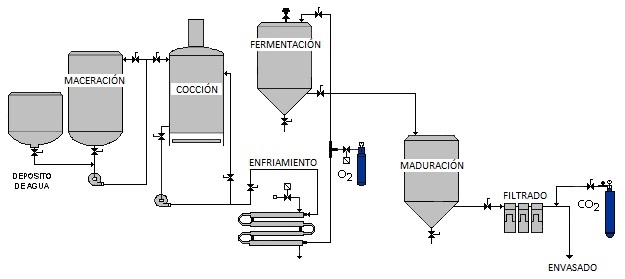
\includegraphics[scale=0.75]{introduccion/Etapasdelproceso.jpg}}
		\caption{Proceso productivo de siete etapas para la elaboración de cerveza: \textit{maceración, cocción, enfriamiento, fermentación, maduración, filtrado y envasado.}}
	    \label{ProcFab}
	\end{figure}
	
	%% --- Arranca con maceración puntualmente 
	\par
	De todas las etapas antes mencionadas, el macerado es el proceso que reviste interés en este proyecto, ya que durante éste el preparado es susceptible a modificaciones de manera de asegurar el resultado deseado. Como explica \cite{Papazian} “El proceso es continuado durante un período de tiempo con ajustes controlados de las temperaturas y pH que activa diferentes enzimas para descomponer los almidones solubles y las proteínas”. Estos ajustes requieren de una atención intensiva durante el proceso por parte del productor, y por tanto, la mayoría de estos no llevan a cabo estas prácticas. Los productores usualmente emplean una única medición de temperatura y pH realizada al inicio del proceso, involucrando en este momento todos los ajustes necesarios y presumiendo que estos valores no se modificaran durante el resto de la maceración.
	\par
	La activación de enzimas presentes en la malta toma un papel protagonista durante el proceso de maceración. El hecho de que las mismas se activen y el grado en el que lo hacen determina el nivel de aprovechamiento de la materia prima utilizada. La calidad del mosto resultante se mide en relación a la densidad del mismo al final del proceso. Cada receta de cerveza conlleva un valor de densidad a ser obtenida, desvíos por encima o por debajo devienen en malos resultados del proceso. Esta densidad objetivo determina la cantidad de insumos (kilogramos de malta) a ser utilizados. Por tanto, realizar un correcto monitoreo del proceso, buscando de esta manera asegurar las condiciones dentro de las cuales las enzimas son activadas es vital para el cumplimiento de los objetivos del proceso de maceración.
	
	\par
	Otro factor determinante en el resultado de densidad, proviene del cálculo de la cantidad de insumos a ser utilizados. En este cálculo, es utilizado un valor que representa la capacidad que tiene el equipo de producción (tanques maceradores) para extraer los subproductos de la malta de forma de cumplir el objetivo de densidad para el proceso. Los productores utilizan un valor genérico para este cálculo, no realizando así el correspondiente ajuste a las características de su equipo. En forma consecuente, los valores obtenidos del cálculo de insumos se alejan de la cantidad necesaria a ser utilizada para un equipo específico.
	
	%% --- Subtitulo, como los cerveceros medianos/chicos llevan adelante el proceso de maceración.
	\subsection{Proceso de macerado en producciones de pequeña a mediana escala }
    
    \par
    A partir de entrevistas a productores, de pequeña y mediana escala, pudieron identificarse los insumos y métodos de maceración que estos utilizan. A continuación, se describen las categorías identificadas.
    
    \subsubsection{Productores de pequeña escala (Aficionados)}
    Pertenecen a esta categoría aquellos productores cuya inversión en equipamiento es baja o reducida. Su objetivo no es el rédito económico, sino, la experiencia de producir cerveza.
    \par
    A continuación se listan los utensilios comúnmente utilizados por estos productores: 
    \begin{itemize}
        \item Conservadora u olla de maceración.
        \item Balanza
        \item Termómetro de mercurio.
        \item Bolsa para macerado
        \item Tinta de Yodo
    \end{itemize}
    
    \paragraph{Procedimiento: } 
    El proceso inicia con la preparación de la cantidad de malta y el calentamiento de agua. Por lo general, se utiliza una relación de tres litros de agua por cada kilo de grano. La temperatura de agua empleada es de 72°C aproximadamente, para que la temperatura de maceración alcance el rango de 66 a 68 °C cuando se mezcle con el grano.
    \par
    Finalizada la preparación preliminar, se incorpora el grano malteado en la conservadora contenido dentro de la bolsa de macerado y luego se vierte el agua caliente dentro de la misma. Posteriormente, se coloca la tapa de la conservadora con el objetivo de aislar térmicamente la mezcla. 
    \par
    El proceso termina luego de una hora aproximadamente. En este momento, se realizan las pruebas con tinta de yodo con la finalidad de verificar que el proceso se haya concretado correctamente, siendo necesario la prolongación del proceso en el caso que este resultado sea negativo.
    \par 
    Para finalizar, se extrae el mosto obtenido en otro recipiente donde será hervido. El volumen de producción usualmente no supera los veinte litros.
    %--------------------------------------------------------------------------------
    %   FALTAN PONER LOS PROBLEMAS DE ESTAS APROXIMACIONES
    %--------------------------------------------------------------------------------
    
    % Conservadoras
    % Tiempo: 1 hora, sin cambio de temperatura objetivo
    % Termómetro manual / medición al inicio.
    % Bolsa de macerado (filtro)
    % No se mide pH (o Si)
    % Prueba de Iodo para saber que termino el proceso
    % Recirculado? Sparring?
    % Palo revolvedor
    % Sales / ácidos diabólica@s para modificar pH que no había dicho bigote en el parador de birras
    
    
	%% aparte de decir como lo hacen, hay que puntualizar que problemas conllevan esas metodologías.
    \subsubsection{Productores de mediana escala}
    Pertenecen a esta categoría aquellos productores que realizan una inversión media en equipamiento, que les permite alcanzar un nivel preindustrial. Su objetivo es el rédito económico.
    A continuación se listan los utensilios comúnmente utilizados por estos productores: 
    \begin{itemize}
        \item Olla de maceración (400 - 1000 litros).
        \item Balanza industrial
        \item Termómetro digital.
        \item Medidor digital de pH.
    \end{itemize}
    \paragraph{Procedimiento: }
    La secuencia de pasos es idéntica a la descripta para los productores aficionados. Se respeta la relación de cantidad de agua por kilogramo de grano, la duración, y la temperatura de maceración antes mencionados. La variación principal se corresponde a un proceso en el cual se trabaja con mayor volumen y mejor calidad de instrumentos.
    \par
    Las ollas de maceración utilizadas cuentan con falso fondo, que sustituye la bolsa de maceración y facilita el proceso de recirculado\footnote{Recirculado: Subproceso del macerado, tiene el fin de extraer los azucares remanentes en el grano al concluir el macerado. Se toma agua del fondo y se la vuelve a agregar por la parte superior del tanque.}. Además, son utilizadas bombas hidráulicas que facilitan el desplazamiento de las mezclas.
    \par
    Para el control del proceso, se verifican los valores de temperatura y pH. La temperatura del agua es controlada previo al inicio del macerado y, una vez vertida dentro de la olla de maceración, no se la vuelve a controlar debido a la confianza de los productores en el aislamiento térmico. En el caso del pH, se realiza una única medición donde se comprueba que el valor del empaste sea de 5.4, siendo aplicada alguna corrección con sustancias químicas en caso de un desvío respecto a dicho valor.
    % higienización de los instrumentos?
    \par
    Al alcanzar la duración de una hora, se da por finalizado el proceso de macerado. Para finalizar, se extrae el mosto obtenido para el siguiente proceso.
    
    
    %olla con falso fondo de 416l, 85/100kg de malta en 3 a 1, agua a 73 grados preparada y al agregar la malta va a 68. ph barato 5.4, temperatura 1 o 2 veces, buen aislante asumen mantenimiento de temp. el ph es solo el del agua antes de preparar
    
    %5.4 ph = barato
    %1 hora
    %67
    
    
    % 416 litros de producción
    
	
	
	%% --- Propuesta de solución ---
	\subsection{ Propuesta de solución }
	\par
    Dentro de este contexto, se propuso el desarrollo de un prototipo de hardware y software para asistir al productor de cerveza artesanal, de escala media y baja, en el proceso de maceración. Esta herramienta proveerá asistencia a través de la planificación de procesos, monitoreo de variables mediante sensores, estimación de variables de control y análisis intensivo de variables intervinientes y sus relaciones.
    \par
    Esta herramienta brinda al productor facilidad para realizar el seguimiento de la evolución del proceso, permitiendo identificar los momentos apropiados donde realizar acciones correctivas. Comportándose las variables (pH y temperatura) según lo esperado en los distintos períodos de la maceración, se evitan resultados disímiles entre diferentes maceraciones y se optimiza la utilización de la malta a través del control puntual de las actividades enzimáticas, derivando en una disminución de insumos y costos.
    \par
    De forma adicional, el sistema provee la capacidad de calcular un valor ajustado, con cada experimento de maceración, de la cantidad de insumos necesaria a ser utilizada para una receta particular. Este ajuste es realizado a partir de un cálculo, repetido en cada experimento de maceración, mediante el cual se obtiene el rendimiento del equipo.
    
\section{Estado del arte}
\label{seccionEstadoDelArte}
    \par
    Se considera de importancia presentar el contexto tecnológico del sistema presentado en este proyecto. Por tanto, a continuación se expone una selección de tecnologías electrónicas e informáticas para asistir al productor de cerveza artesanal. Estas son clasificadas en tres grupos según el tipo de aproximación que cada solución utiliza.
    
    \par
    \textbf{Sistemas informáticos basados en software:} Las herramientas identificadas en este grupo comparten un abordaje común hacia la temática, ya que todas implementan como base un registro de recetas (con diferentes niveles de detalle). De forma adicional incorporan una serie de utilidades, llamadas calculadoras, cuyo fin es la estimación de medidas, tiempos y cantidades de insumos intervinientes en el proceso de elaboración de cerveza artesanal. A continuación, se realiza mención a dichos aplicativos de software:
    \begin{itemize}
        
        \item {\textit{BeerSmith}\textsuperscript{®}}: Este sistema cuenta con un registro de alta especificación técnica para detallar elementos y variables intervinientes en el proceso de fabricación de cerveza artesanal. De forma adicional, incorpora un gran repertorio de calculadoras de estimación de valores para diversos fines.
        \par
        Utilidad para el proceso de maceración: Registro detallado de insumos intervinientes en el proceso, provee calculadoras específicas: ``Mash Adjust'' su fin es el cálculo de las adiciones de agua necesarias para lograr un objetivo de temperatura de maceración; ``Mash pH'' cuyo objetivo es la estimación de cantidades de sales necesarias para ajustar el pH de un mosto.
        \par
        \textit{Beersmith}\textsuperscript{®} es un software para computadora en idioma inglés que funciona sobre los sistemas operativos Windows\textsuperscript{®},Linux y macOS\textsuperscript{®}. Debe ser pagarse una licencia para su utilización.
        \par
        Licencias: Ofrece licencias por tiempo limitado cuyo valor varía entre los 15 USD y 50 USD.
        
        \item{\textit{BrewersFriend}\textsuperscript{®} }: Herramienta de software para asistencia en la producción de cerveza cuya principal funcionalidad es un registro de recetas con detalle de insumos y variables intervinientes en el proceso de fabricación. Incorpora calculadoras de estimación de diferentes valores intervinientes en el proceso de fabricación de cerveza. De forma adicional ofrece a sus usuarios la posibilidad de compartir recetas y experiencias a través de una red social propia.
        \par
        Utilidad para el proceso de maceración: Registro de insumos intervinientes en el proceso, provee las siguientes calculadoras específicas: ``Mash Calculator'' cuyo objetivo es calcular la temperatura del agua a ser agregada a la malta para alcanzar una temperatura deseada; ``All Grain OG/FG'' es una calculadora para estimar densidades de control a ser obtenidas al final de las etapas de maceración y fermentación.
        \par
        \textit{BrewersFriend}\textsuperscript{®} es una aplicación de plataforma web en idioma inglés, que ofrece licencia comercial para su utilización.\\
        Licencias: Ofrece una licencia por tiempo limitado con un costo de 25 USD.
        
        \item{\textit{Brew-O-Matic}}: Herramienta de software cuyo fin es brindar un registro de recetas de cerveza artesanal para usuarios con conocimientos básicos sobre la temática. De forma adicional, brinda a través de su plataforma, una red social de productores de cerveza artesanal. En esta red, los usuarios pueden compartir recetas y realizar colaboraciones sobre recetas con otros productores.
        \par
        Utilidad para el proceso de maceración: Registro de insumos.
        \par
        \textit{Brew-O-Matic} es una aplicación de plataforma web en idioma español, desarrollada en Argentina, que ofrece licencia gratuita para usuarios registrados.
        
    \end{itemize}
    \par
    \textbf{Herramientas de Hardware:}
    Las herramientas identificadas en este grupo, brindan prestaciones en medición de características físico-químicas de las soluciones intervinientes en el proceso de fabricación de cerveza. Adicionalmente, permiten la comunicación de los datos digitales obtenidos de las mediciones a través de diferentes interfaces. A continuación, se realiza mención a dichas herramientas:
    \begin{itemize}
        \item \textit{Tilt}\textsuperscript{®}: Esta herramienta consta de un encapsulado electrónico sumergible capaz de realizar mediciones de densidad y temperatura. La misma posee interfaz inalámbrica a través de la cual se conecta a una aplicación para smartphones para su control. De forma adicional, provee software para ser instalado en una RaspBerry\textsuperscript{®} Pi cuyo fin es conectarse a un dispositivo Tilt\textsuperscript{®} y transmitir datos de las mediciones realizadas a una hoja de cálculo de Google\textsuperscript{®} u otras herramientas de software como por ejemplo, la antes mencionada,  BrewersFriend\textsuperscript{®}.
        \par
        Utilidad para el proceso de maceración: Esta herramienta fue diseñada para ser usada durante el proceso de fermentación, sin embargo, sus capacidades son de utilidad para realizar mediciones de ciertas variables inherentes al proceso de maceración.
        \par
        Costo de adquisición: 135 USD.
        
        \item{\textit{SmartPid}\textsuperscript{®}}: Este dispositivo consiste de un controlador electrónico para sensores de temperatura. Posee un interfaz que cuenta de una pantalla y una serie botones para este fin que permiten interactuar con el mismo, además puede ser conectado a una aplicación móvil provista por el fabricante.
        \par
        Utilidad para el proceso de maceración: Permite llevar a cabo un monitoreo estricto de la temperatura. 
        \par
        Costo de adquisición: 140 USD.
        
    \end{itemize}
    \par
    \textbf{Sistemas para monitoreo de mediciones:}
    Las herramientas identificadas en este grupo tienen como propósito llevar adelante el monitoreo de variables intervinientes en el proceso de fabricación de cerveza artesanal. Constan de un componente controlador de software e integraciones con hardware para recolección de mediciones.\\
    A continuación se mencionan las mismas:\\
    \begin{itemize}
    
        \item \textit{BruControl}\textsuperscript{®}: Este sistema se divide en dos partes, un componente de software y un componente de hardware. El componente de software es una aplicación de escritorio cuya funcionalidad varía según el nivel de conocimientos de programación que posee el usuario: Usuario sin conocimientos de programación, la aplicación solo muestra en pantalla los valores medidos provenientes del componente de hardware; Usuario con conocimientos de programación, permite configurar alertas y tomar acciones reactivas, por ejemplo, encender una resistencia para calentar un tanque debido a la pérdida de temperatura de la solución. Componente de Hardware, placas electrónicas de tipo Arduino a las cuales se le conectan distintos tipos de sensores.
        \par
        El fabricante provee tanto la aplicación de software como los componentes electrónicos.
        \par
        Utilidad para el proceso de maceración: Asiste en el monitoreo de las variables intervinientes en el proceso.
        \par
        Costo de adquisición: Las licencias de software varían entre los 119 USD y 200 USD según la cantidad de conexiones electrónicas a ser incorporadas. Los componentes de hardware varían en precio según la funcionalidad, el fabricante permite y ofrece la integración del software con hardware de terceros.
        
        \item \textit{CraftBeerPi}\textsuperscript{®}: Este sistema, implementado sobre Raspberry Pi, permite el control de la producción a través de una interfaz web.
        Las características que posee este sistema son: Control de temperatura mediante sensores digitales; control de actuadores; reproducción de sonidos para indicar eventos durante la producción; visualización y activación de actuadores mediante su interfaz web.
        \par
        Enfocándose en la maceración, el control de temperatura y la reproducción de sonidos permite evaluar que la temperatura sea adecuada al proceso planificado dentro de la duración definida para el proceso.\\
        Utilidad para el proceso de maceración: Monitoreo de temperatura durante el proceso.
        \par
        Costo de adquisición: El sistema es de código abierto y bajo licencia gratuita. El fabricante no provee los componentes electrónicos para la implementación del sistema.
        
    \end{itemize}
    
    % Especie de conclusión.
    Puede concluirse, que existen tres enfoques que toman los desarrolladores asistir al productor de cerveza: 
   
    \begin{enumerate}
            \item Registro de recetas y utilidades para diferentes de cálculos.
            \item Herramientas de hardware para medición de valores.
            \item Sistemas mixtos para medición y monitoreo de variables de importancia.
    \end{enumerate}

\section{Objetivos}
\label{secccionObjetivos}
    \par
    A continuación se presentan los objetivos para el desarrollo de este proyecto. Divididos en objetivos generales y específicos.

    %\subsection{Objetivos generales}
    \subsection{Objetivo general}
        \par
        Desarrollar un prototipo de hardware y software para asistir al productor de cerveza artesanal en la planificación, seguimiento y evaluación del proceso maceración. 
    \subsection{Objetivos específicos}
        \begin{itemize}
            \item Analizar, diseñar y construir un sistema electrónico para la medición mediante el sensado de las variables intervinientes en el proceso de maceración.
            
            \item Desarrollar una aplicación móvil que brinde funcionalidades que faciliten la planificación, seguimiento y evaluación del proceso de maceración.
            
            \item Analizar, desarrollar, aplicar y utilizar una interfaz como medio de comunicación entre el sistema electrónico y la aplicación móvil.
            
            \item Ensamblar y validar el prototipo como una construcción del sistema electrónico, la aplicación móvil y la interfaz.
        \end{itemize}
 
\section{Alcance}
    \par
    En este apartado se presenta el alcance del proyecto, el cual fue definido en etapas previas\footnote{Este alcance fue definido en el documento de Anteproyecto} al desarrollo del prototipo. En este son incorporadas las inclusiones, exclusiones y supuestos que fueron considerados.
    \par
    Se desarrollará un prototipo de hardware y software compuesto por un sistema electrónico y una aplicación móvil. El primero estará formado por un conjunto de sensores ubicados en diferentes puntos que medirán los valores de temperatura y pH del preparado. Por otra parte, un controlador transmitirá a través de una interfaz los valores sensados. La aplicación, por su parte, se encargará de brindar las funciones de planeamiento de procesos de maceración, simples y complejos, incorporando estimación de variables de control, configuración de estrategias de obtención, monitoreo y notificación de desvíos de medidas, registro histórico de procesos, visualización gráfica, análisis estadístico y comparativo de la evolución temporal de variables intervinientes en diferentes maceraciones a partir de muestras puntuales, medidas representativas o valores ingresados.
    \par
    El sistema será desarrollado para un usuario con conocimientos teóricos suficientes que pueda entender y relacionar la información presentada, y reaccionar en consecuencia si el proceso lo requiere. El usuario será responsable del ingreso manual de datos de insumos, medidas de densidad, y comienzo y fin del proceso en la aplicación móvil.
    \par
    El desarrollo no proveerá un sistema automatizado de macerado ni una planificación, seguimiento y evaluación del proceso, sino que proveerá datos útiles y fidedignos a través de sus funcionalidades para asistir en dichas actividades. El prototipo propuesto será funcional, cumplirá las características previamente mencionadas sin alcanzar la etapa de implementación.
    \par
    Se da por aceptado que el dispositivo móvil cuenta con los servicios Wi-Fi y Bluetooth funcionando en forma correcta y operando con una versión actual del sistema operativo o de no más de un año de antigüedad en relación a la fecha de este desarrollo. En caso de utilizar conexión Wi-Fi para la interfaz, se deberá disponer de un dispositivo de red Router para el establecimiento de una red local y se configurarán los parámetros de red del sistema electrónico en forma manual.
    \par
    La precisión de los valores medidos difiere según la calidad de los sensores. Como se propone el desarrollo de un prototipo, los mismos pueden no ser exactos y no se realizará un análisis en profundidad en relación a este nivel de precisión. 
    \par
    Se deja para un futuro desarrollo la posibilidad de supervisar múltiples maceradores simultáneamente. 
 
\section{Metodología}

    \par
    En este apartado se presenta la metodología utilizada para el desarrollo del presente proyecto.
    \par La metodología seleccionada para este proyecto es la de ciclo de vida en cascada enmarcando el desarrollo completo del sistema. En el mismo, cada proceso es secuencial y la finalización de uno de ellos es el punto de inicio del siguiente.
    
    \par Al finalizar cada etapa se presenta un hito, que es el resultado de la etapa, el cual está sujeto a determinados criterios de aceptación. En cada etapa, el director del proyecto es quien juzga si los resultados obtenidos satisfacen estos criterios.

    \paragraph{Etapas:}
        \begin{enumerate}
            \item Análisis temático y de requerimientos:
                \par En la etapa inicial se realiza una investigación bibliográfica, enfocada en el estudio del procedimiento de fabricación de cerveza artesanal, con especial atención en los procesos y subprocesos del macerado. Se redacta en forma adicional un análisis de requerimientos para el proyecto. Al finalizar esta etapa se documenta el análisis temático que contendrá las bases teóricas que sustentan este proyecto.
                \par \textit{Hito 1: Adquisición de conocimientos necesarios.}
                
            \item Análisis, diseño y desarrollo del componente Hardware:
                \par Se lleva a cabo una investigación y análisis de potenciales soluciones para el abordaje del hardware, luego se  documenta esta investigación y se justifica la elección de la solución. Luego, se realiza un aprendizaje de desarrollo de la tecnología utilizada en la solución, para en forma consecuente, realizar el diseño y desarrollo de este sistema.
                \par \textit{Hito 2: Sistema electrónico desarrollado.} 
                
            \item Análisis, diseño y desarrollo del componente Software:
                \par En esta etapa, se realiza una investigación y análisis de potenciales tecnologías móviles a utilizar que son documentadas junto a la elección de mayor conveniencia para esta etapa. A continuación, se lleva a cabo un aprendizaje de desarrollo de aplicaciones en esta tecnología, para en forma consecuente, producir el diseño y desarrollo de la aplicación.
                \par \textit{Hito 3: Aplicación móvil desarrollada.}
                
            \item Análisis, diseño y desarrollo de la Interfaz Hardware - Software:
                \par Se entiende a la interfaz como un espacio donde se desarrolla la interacción y el intercambio entre dos sistemas. Disponiendo del sistema de hardware y la aplicación móvil, se realiza una investigación y análisis de posibles alternativas, procediendo a continuación con el desarrollo de la misma.
                \par \textit{Hito 4: Interfaz desarrollada.}
                
            \item Integración y ciclo de pruebas:
                \par Se realiza la integración de los desarrollos y un ciclo de pruebas de campo para corroborar el correcto funcionamiento del sistema. Por último, se concreta con la redacción del informe final del proyecto.
                \par \textit{Hito 5: Proyecto Finalizado.}

        \end{enumerate}